\chapter{Part 1: Synchronization of Extreme Events}
\label{c:event_sync}
During the primary monsoon season, floodings and landslides caused by extreme rainfall can lead to massive societal and environmental damage \citep{Stolbova.2015}. It is thus crucial to be able to analyze, detect and potentially predict such extreme rainfall events, especially as their proportion tends to further increase with global warming \citep{Stolbova.2015} [TODO: cite Goswami?].

A way of analysis that \citet{Stolbova.2015} has proposed is the computation of climate networks based on different locations in India, followed by an analysis of the resulting networks using graph centrality measures. We strongly base this chapter on her work and thus summarize her approach in \cref{sst:event_sync}. We also explain the network measures that will be applied to the resulting climate networks (\cref{sst:network_measures}) and introduce the dataset that will be used as a basis for all calculations (TRMM, \cref{sst:trmm_dataset}).

\cref{st:event_sync_implementation} then provides an overview of our approach to the creation of climate networks and explains where our approach differs from the work of \citep{Stolbova.2015}. Following up in \cref{st:event_sync_results}, we analyze and visualize the computed climate networks using graph centrality measures and try to interpret the results in contrast to the known factors of monsoon behavior. Concluding this chapter in \cref{st:event_sync_conclusion}, we elaborate the usefulness of our results and how they could be improved upon.

\section{Related Work}
[TODO: need text here?]

\subsection{The TRMM dataset}
\label{sst:trmm_dataset}
The Tropical Rainfall Measurement Mission (TRMM) is a precipitation research effort by the National Aeronautics and Space Administration (NASA) and the Japanese Aerospace Exploration Agency (JAXA). It is based on the TRMM observatory, a satellite that was launched into space on the 27th of November, 1997. The products based on TRMM range from the raw output of the multitude of sensors on the satellite to the highly aggregated and gridded rainfall estimates we will be using in this work \citep{GoddardEarthScienceDataInformationandServicesCenter.2016}.

More specifically, the TRMM product that we will be using is a 3-hourly estimate of surface rainfall aggregated from the satellite sensors in combination with surface gauge values and imagery from other satellites. This product is referred to as 3B42 or TMPA and is also available in a daily variation, where the eight 3-hourly measurements (i.e., 00:00, 03:00, 06:00 and so on) have been summed up to provide a single daily rainfall estimate.

[TODO: update coordinates and grid specifics] 3B42 is available for the area between 50\degree N. and 50\degree S. We subset this area to cover the entire Indian subcontinent (x-x\degree N, x-x\degree E). These border coordinates are a superset of the ones used in \citep{Stolbova.2015}: the grid has been extended  such that it can be cleanly aggregated from a 0.25\degree spatial resolution to the 0.75\degree resolution of the ERA-Interim dataset (which we will use later on). \cref{fig:trmm_area} shows the excerpt of the TRMM dataset that we will be using in this work.

\begin{figure}[h]
  \centering
  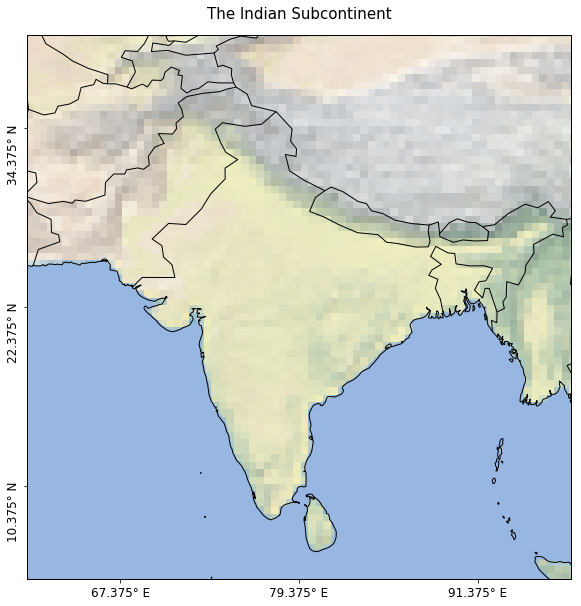
\includegraphics[width=0.5\linewidth]{./99_appendix/img/area_overview}
  \caption{The Indian subcontinent as extracted from TRMM.}
  \label{fig:trmm_area}
\end{figure}

The TRMM dataset is unique in that it offers very high-resolution precipitation estimates since January 1998. It can prove useful for research based on the distribution, frequency, and intensity of rainfall, i.e., for calculating extreme rainfall events \citep{Stolbova.2015}. However, it has to be taken into consideration that the TRMM products are based on complex algorithms and have been derived from different sensors and sources \citep{Huffman.2017b}.

After the TRMM satellite's fuel went low in 2014, it was decommissioned in April 2015 and re-entered earth's atmosphere in June 2015. The TMPA product is still being produced until 2018, albeit without the sensors of the TRMM observatory and with less accuracy \citep{Huffman.2017}.

Built on the success of the TRMM mission, NASA and JAXA have launched its successor GPM (Global Precipitation Measurement) in 2014 \citep{GoddardEarthScienceDataInformationandServicesCenter.2011}. However, as its data is only available starting from 2014, GPM is currently unsuitable for long-term precipitation research. TRMM or an alternative dataset are currently still needed but the updated algorithm developed for GPM will soon be applied to the existing TRMM data. The availability of reprocessed data back to 1998 can thus be expected in 2018 \citep{Huffman.2016}.


\subsection{Event synchronization \& climate networks}
\label{sst:event_sync}
The concept of event synchronization applied in \citet{Stolbova.2015} as well as in our work was first defined in \citet{QuianQuiroga.2002}. \citet{QuianQuiroga.2002} sought to develop a simple algorithm that could be applied to any two time series of events, resulting in a measure that defines the synchronization of said time series. Synchronization measures are generally related to standard measures like cross correlation. They can, however, convey more complex relationships due to their non-linearity \citep{QuianQuiroga.2002}.

\subsubsection{Basic event synchronization}
The basic principle of the event synchronization measure as found in \citet{QuianQuiroga.2002}, \citet{Malik.2010} and \citet{Stolbova.2015} is setup as follows: given the two time series $i$ and $j$ and their respective events $l$ and $m$ occuring at times $t^i_l$ and $t_j^y$, we measure the synchronicity for all possible pairs of events between both series. We classify events as synchronous if they occur closely simultaneous, i.e., within a certain range from each other. This allowed range of occurrence is called \textit{time lag} and is calculated by taking the minimum interevent distance $\tau^{ij}_{lm}$ like so\footnote{If event rates were fixed, a global time lag $\tau$ could be defined, greatly simplifying calculations.}:

\begin{equation}
\tau^{ij}_{lm} = 0.5 * min\left\{t^i_{l+1} - t^i_l, t^i_l - t^i_{l-1}, t^j_{m+1} - t^j_{m}, t^j_{m} - t^j_{m-1}\right\}
\end{equation}

The synchronicity $J$ of any two events $t_i^x$ and $t_j^y$ is then calculated as follows:

\begin{equation}
  J_{ij} =
  \begin{cases}
    1, & \text{if } 0<t^x_i-t^y_j\leq\tau_{ij}, \\
    0.5, & \text{if } t^x_i=t^y_j, \\
    0, & \text{else.}
  \end{cases}
\end{equation}

Applying this to the full time series $i$ and $j$, the number of synchronous events where an event in $i$ leads an event in $j$ is defined like:

\begin{equation}
  c(i \mid j) = \sum\limits^{s_i}_{l=1} \sum\limits^{s_j}_{m=1} J_{ij}
\end{equation}

The same formula applies to the reversed situation, i.e. $c(j \mid i)$, with $s_i$ and $s_j$ being the number of events in the respective time series. Combining the results of $c(i\mid j)$ and $c(j \mid i)$ and normalizing them by the total numbers of events $s_i$ and $s_j$, the \textit{strength of synchronization} is defined as

\begin{equation}
  Q_{ij} = \frac{c(i \mid j) + c(j \mid i)}{\sqrt{(s_i - 2)(s_j - 2)}}
\end{equation}

where $Q_{ij} = 1$ means that the time series are completely synchronized, i.e., that each event in $i$ is either synchronously lead or followed by an event in $j$.

\subsubsection{Application to climate networks}
\label{ssst:appl_climate_networks}
While the work of \citet{QuianQuiroga.2002} focuses on the analysis of EEG\footnote{EEG: Electroencephalogram; A way of measuring brain activity.]} time series, their event synchronization approach is explicitly applicable to other domains. The works of \citet{Malik.2010} and \citet{Stolbova.2015} both expand upon simple event synchronization. For the purposes of our work, we focus on the approach using climate networks as found in \citet{Stolbova.2015}.

Looking at the TRMM dataset as shown in \cref{fig:trmm_area}, each cell of its coordinate grid represents a separate precipitation time series. As the analysis of each monsoon season is performed seperately, one such coordinate grid per season needs to be extracted\footnote{The time series are then simply the respective months of each year, concatenated into a single series.}.

The time series in the resulting grids are not event based and thus cannot be directly used to calculate synchronization. They can, however, easily be transformed into event series by extracting only the days where extreme rainfall occurred. As per \citet{Stolbova.2015}, such days are generally defined as days with rainfall that exceeds the 90th percentile for the respective location.

The resulting series of extreme events can be used to calculate the synchronicity of different locations (grid cells) in the TRMM dataset. Computing the synchronicity for all possible permutations of two such locations then results in a synchronization matrix as can be seen in \cref{fig:synchronization_matrix}.

\begin{figure}[h]
  \centering
  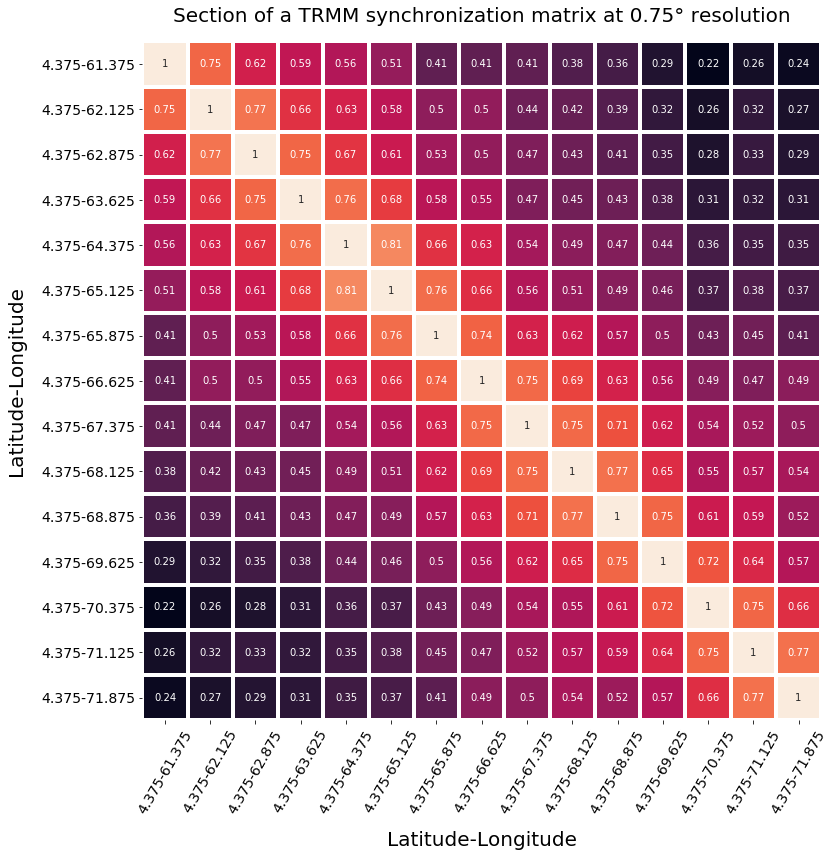
\includegraphics[width=0.65\textwidth]{./99_appendix/img/trmm_sync_example}
  \caption{Exemplary synchronization matrix for TRMM at a 0.75\degree resolution. We only show the top left 15x15 section of our actual matrix, as its full dimensions are 2401x2401 for a 0.75\degree resolution.}
  \label{fig:synchronization_matrix}
\end{figure}

Applying a numerical threshold to this synchronization matrix results in a matrix that contains only the most significantly synchronous values. Everything else is set to zero, including the diagonal of the matrix, as this would result in loops in the graph later on. Additionally, all elements above the threshold are set to one, yielding the adjacency matrix for an undirected, unweighted network (\cref{fig:adjacency_matrix}). \citet{Stolbova.2015} uses the 95th percentile for the threshold applied, as this removes all but the most statistically significant values.

\begin{figure}[h]
  \centering
  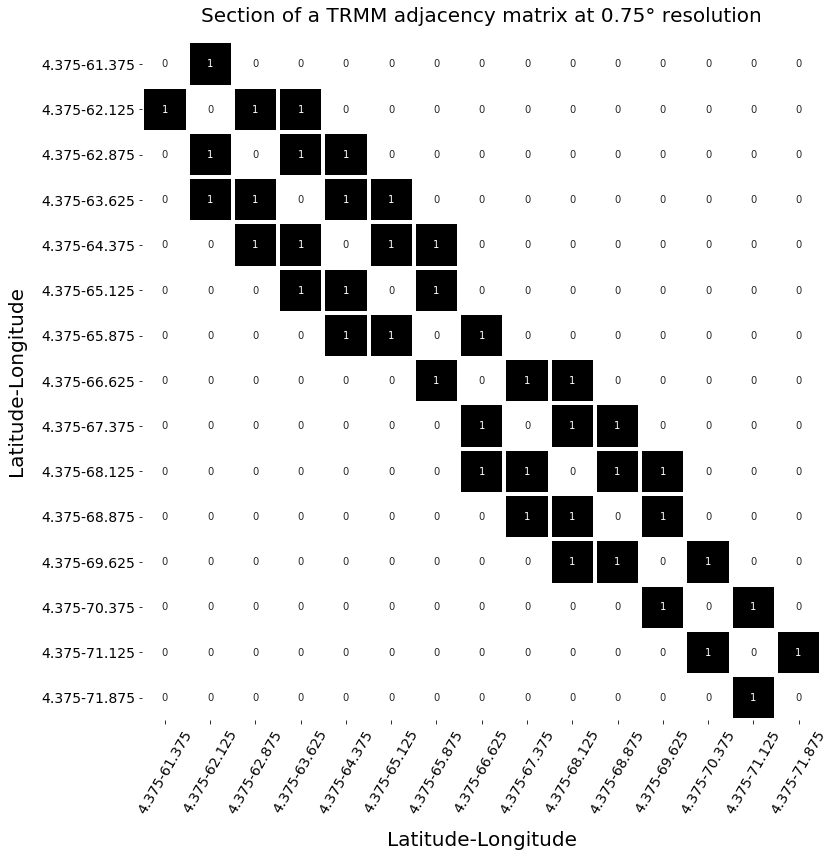
\includegraphics[width=0.65\textwidth]{./99_appendix/img/trmm_adjacency_example}
  \caption{Exemplary adjacency matrix for TRMM at a 0.75\degree resolution. We only show the top left 15x15 section of our actual matrix, as its full dimensions are 2401x2401 for a 0.75\degree resolution.}
  \label{fig:adjacency_matrix}
\end{figure}

Based upon the adjacency matrix, a network can then be computed and analyzed. However, before we detail our implementation of it, the next section briefly describes the measures that we will be using for said network analysis.

\subsection{Graph centrality}
\label{sst:network_measures}
Constructing climate networks from an adjacency matrix as seen in \cref{ssst:appl_climate_networks} enables the analysis of their structural features using various graph-based measures. We now shortly go over the concepts of the measures that we apply to our networks in this work.

The climate networks in \citet{Stolbova.2015} are analyzed using the \textit{degree} and \textit{betweenness} of nodes as well as using the \textit{average/maximal geographical link length} between them. We also base our analysis on the \textit{degree} and \textit{betweenness} measures but replace the link length calculations with the PageRank algorithm, which could, in our opinion, show more distinct patterns than the other two measures.

The \textit{degree} of a node in a network is quite simply defined as the amount of links that are connected to the respective node. The same holds for vertices in graphs and their connected edges.

Calculating the \textit{betweenness} or \textit{betweenness centrality} of a node is a more involved effort. A node has a high betweenness if a large portion of shortest paths in the network pass through the respective node. If the resulting betweenness is to be an exact measure, this basically necessitates the calculation of all shortest paths in the network, which gets increasingly complex with the size of the graph. There are, however, algorithms that achieve both accuracy and speed when calculating betweenness, one of the most popular being the approach proposed by \citet{Brandes.2001}\footnote{This algorithm is also used by the Python library \textit{networkx}, which we will be using for our calculations.}.

The final measure that we will apply to climate networks, the \textit{PageRank} algorithm, was originally developed and published by the founders of Google (amongst others), Larry Page and Sergey Brin, during their studies at Stanford University \citep{Page.1999}.

[TODO: finish page rank]

\section{Implementation}
\label{st:event_sync_implementation}
Our implementation of the event synchronization and climate network computations is strongly based on the concepts and measures as described in \cref{sst:event_sync} and \cref{sst:building_climate_network}. As our algorithmic implementation is most certainly different than the one used in the original work \citep{Stolbova.2015}, we shortly go over our approach to the problem in this section.

\subsection{Calculating event synchronization}
\label{sst:event_sync_calculation}
Before we are able to calculate the synchronicity for any two locations, the precipitation time series need to be transformed into series of events. Assume that we have extracted pre-monsoon time series as shown in \cref{tab:example_rainfall_ts} from the TRMM dataset and now want to convert these into extreme event series.

\begin{table}[h]
  \centering
  \begin{tabular}{ |c|c|ccccccc| }
    \hline
    Latitude & Longitude & 01.03.98 & ... & 29.05.98 & 30.05.98 & 31.05.98 & 01.03.99 & ...\\
    \hline
    13.375 & 67.375 & 0.0  & ... & 0.12 & 2.31  & 2.85  & 0.00 & ... \\
    16.375 & 91.375 & 0.0  & ... & 0.09 & 34.80 & 49.49 & 0.00 & ... \\
    34.375 & 67.375 & 0.52 & ... & 0.00 & 0.00  & 0.00  & 0.00 & ... \\
    34.375 & 88.375 & 0.86 & ... & 2.01 & 51.85 & 68.72 & 0.29 & ... \\
    \hline
  \end{tabular}
  \caption{Precipitation time series during pre-monsoon at 4 exemplary locations (TRMM, 0.75\degree).}
  \label{tab:example_rainfall_ts}
\end{table}

We calculate the 90th percentile seperately for each row and apply the result as a threshold to the respective row. This yields event series where each value represents the date of an extreme event in the series. This would look as shown in \cref{tab:example_rainfall_events} if applied to the time series in \cref{tab:example_rainfall_ts}.

\begin{table}[h]
  \centering
  \begin{tabular}{ |c|c|ccccccc| }
    \hline
    Latitude & Longitude & 1 & 2 & 3 & 4 & 5 & 6 & ... \\
    \hline
    13.375 & 67.375 & 07.04.98 & 31.05.98 & 08.05.99 & 12.05.99 & 13.05.99 & 15.05.99 & ... \\
    16.375 & 91.375 & 17.05.98 & 18.05.98 & 19.05.98 & 30.04.99 & 01.05.99 & 05.05.99 & ... \\
    34.375 & 67.375 & 03.03.98 & 29.03.98 & 02.04.98 & 03.04.98 & 09.04.98 & 22.04.98 & ... \\
    34.375 & 88.375 & 18.03.98 & 30.03.98 & 31.03.98 & 01.04.98 & 05.04.98 & 19.04.98 & ... \\
    \hline
  \end{tabular}
  \caption{First events in the pre-monsoon extreme event series at 4 exemplary locations (TRMM, 0.75\degree).}
  \label{tab:example_rainfall_events}
\end{table}

With a matrix of extreme events as shown in excerpt in \cref{tab:example_rainfall_events}, we then calculate the event synchronization for all pairs of locations. \cref{tab:example_empty_sync} shows the state of a preliminary synchronization matrix before running any of the calculations. Locations are always perfectly synchronous to themselves, leading to a diagonal that will always be filled with ones.

\begin{table}[h]
  \centering
  \begin{tabular}{ |cc|cccc| }
    \hline
     & Latitude & 13.375 & 16.375 & 34.375 & 34.375 \\
    Latitude & Longitude & 67.375 & 91.375 & 67.375 & 88.375 \\
    \hline
    13.375 & 67.375 & 1 &   &   &   \\
    16.375 & 91.375 &   & 1 &   &   \\
    34.375 & 67.375 &   &   & 1 &   \\
    34.375 & 88.375 &   &   &   & 1 \\
    \hline
  \end{tabular}
  \caption{Empty synchronization matrix for 4 exemplary locations (TRMM, 0.75\degree).}
  \label{tab:example_empty_sync}
\end{table}

To further fill in the values of the synchronization matrix in \cref{tab:example_empty_sync}, our algorithm only needs to perform calculations for one of the now empty halves of the matrix. This is due to the fact that, at least in our approach, the synchronization between two locations can be symmetrically applied to both their permutations. The original work on event synchronization by \citet{QuianQuiroga.2002} describes some asymmetrical measures, that were, however, not used in the work of \citet{Stolbova.2015}.

Having explained the necessary setup of the event synchronization algorithm, we now go into the



[TODO: describe our sliding window approach for event sync calculation]

[TODO: ? describe parallelization and further possible optimizations?]

[TODO: ? go into runtime and O(x) of the algorithm?]

\subsection{Building climate networks}
\label{sst:building_climate_network}
[TODO: describe our approach to building the climate networks]

... Elements above the threshold can either be set to 1 or left at the value of the synchronization coefficient, depending on whether an unweighted or weighted network should be created. ...


\section{Results \& Evaluation}
\label{st:event_sync_results}
[TODO: describe the results that were obtained by our approach]

[TODO: interpret the results, incorporating knowledge of impacting factors]

[TODO: compare the results with stolbova and try to explain differences]

[TODO: refer to appendix for full visualizations]

\section{Conclusion}
\label{st:event_sync_conclusion}
[TODO: conclude the chapter]
